%!TEX TS-program = pdflatex
\documentclass[twoside]{article}
\usepackage{waspaa01,amssymb,amsmath,epsfig}
\usepackage{graphicx,mcode}
\usepackage{listings}
\usepackage{verbatim}
\usepackage{url}

%% Now actually use the newly defined style.

\lstset{ %
%language=C,                % choose the language of the code
%basicstyle=\footnotesize,       % the size of the fonts that are used for the code
%numbers=left,                   % where to put the line-numbers
numberstyle=\footnotesize,      % the size of the fonts that are used for the line-numbers
stepnumber=1,                   % the step between two line-numbers. If it's 1 each line will be numbered
numbersep=0pt,                  % how far the line-numbers are from the code
backgroundcolor=\color{white},  % choose the background color. You must add \usepackage{color}
showspaces=false,               % show spaces adding particular underscores
showstringspaces=false,         % underline spaces within strings
showtabs=false,                 % show tabs within strings adding particular underscores
tabsize=2,                      % sets default tabsize to 2 spaces
captionpos=b,                   % sets the caption-position to bottom
breaklines=true,                % sets automatic line breaking
breakatwhitespace=false,        % sets if automatic breaks should only happen at whitespace
escapeinside={\%*}{*)}          % if you want to add a comment within your code
}
\setcounter{page}{1}
%\ninept  % 9-pt size optional (10-pt default)

\title{Veritune: Auto-Tuning in Verilog}
\name{Chris Li, Grayson Smith, Carey Zhang}
\address{github.com/unregistered/speakurity}

%
\begin{document}
\maketitle
%
\begin{abstract}
	For our EE201 final Verilog project, we implement pitch shifting in hardware.
\end{abstract}

%
%
% Introduction
%
%
\section{Introduction}
  Something on the phase vocoder \cite{bib:guitarpitchshifter}.
  
%
%
% FFT
%
%
\section{Radix-2 DIT FFT}
  The first component we had to create was the Fast Fourier Transform. The FFT takes a discrete signal in the time domain and 
  transforms it into the frequency domain. For our device we need a 1024 point FFT.
  \subsection{Relevant Theory}
  The Discrete Fourier Transform is shown below.
  \begin{equation}
  	X_k = \sum_{n=0}^{N-1} x_n e^{-\frac{2 \pi j}{N} k n} \quad \quad k = 0, \dots, N-1
  	\label{eqn:dft}
  \end{equation}
  
  However, the number of operations required scales as $N^2$ and the DFT becomes very expensive at 1024 points.
  The Cooley Tukey Algorithm is an Fast Fourier Transform, which reduces the number of operations \cite{bib:ctdft}.
  \begin{equation}
  	 X_k  =	 \sum \limits_{m=0}^{N/2-1} x_{2m}     e^{-\frac{2\pi j}{N} (2m)k}\\   +  \sum \limits_{m=0}^{N/2-1} x_{2m+1} e^{-\frac{2\pi j}{N} (2m+1)k}
  	\label{eqn:ctdft}
  \end{equation} 
  
  \subsection{Hardware Implementation}
  Because the number of points is a power of two, we can use Radix-2 Decimation in Time.
  The Cooley Tukey Algorithm can be applied recursively until the size of the FFT is 2.  
  The dataflow for our algorithm is shown in figure \ref{fig:butterfly}.  Each column
  is called a pass, each set of interlocked rows in the pass is a block, and each pair of lines is called a 
  butterfly (after the appearance of crossing lines).
  \begin{figure}[h]
  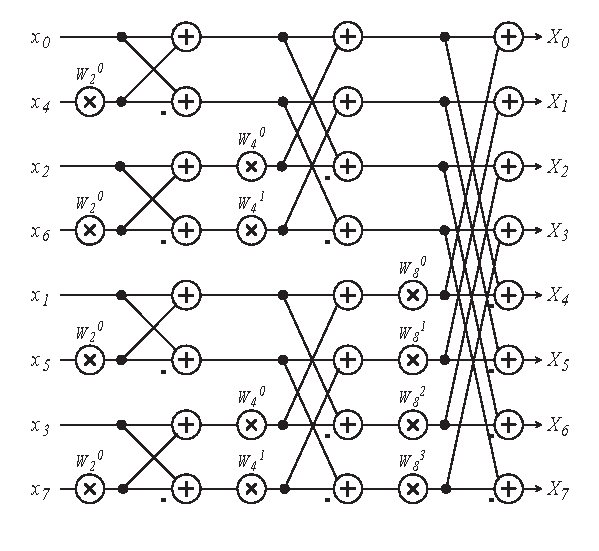
\includegraphics[width=75mm]{images/butterfly.pdf}
  \caption{Dataflow of radix-2 DIT FFT \cite{bib:butterfly}. $W_k^n$ represents the Twiddle factor $e^{-\frac{2\pi j}{N}kn}$.}  
  \label{fig:butterfly}
  \end{figure}
  
  We have chosen this algorithm for the substantial savings in operations. The number of complex multiplies and adds in
  the Radix-2 DIT FFT scales as $Nlog(N)$. In theory, a 1024 point DFT requires 1048576 multiplies while the FFT uses 
  only 5120 \cite{bib:fftdit}.
  
  The FFT requires us to compute a complex exponential, which can be expressed as a sine and cosine.  One option would be to 
  implement CORDIC for calculating trigonometric functions.  However, the exponential is a function of only current indexes.  
  Therefore, we implemented it as a look up table with 512 elements (the function is symmetric).  The elements in the LUT
  are called Twiddle Factors. 
  
  Another feature of this implementation is the bit re-ordering, as shown in the figure. Because the algorithm computes the
  FFT in-place, we must re-order the input data.  On software systems this is less desirable but in hardware we can do this
  in one clock or re-index our data.  The re-ordered index is simply the old order backwards in binary.  As such, 
  10'b0000000001 becomes 10'b1000000000, or 10'd512.
  
  
  
  \subsection{The Inverse Transform}
    After manipulating the signal in the frequency domain, we must transform back into the time domain for playback. 
    Rather than implementing a separate IFFT module, we can reuse the FFT module.  We simply switch the real and imaginary
    inputs and divide the final result, which will be located in the imaginary data, by 1024.

%
%
% Phase vocoder
%
%
\section{Phase Vocoder}
  Something
  \begin{figure}[h]
  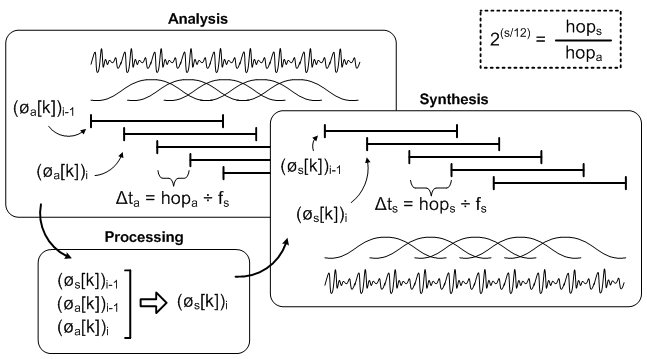
\includegraphics[width=75mm]{images/vocoder.png}
  \caption{Processes involved in a phase vocoder \cite{bib:guitarpitchshifter}.}  
  \label{fig:vocoder}
  \end{figure}

%
%
% Top level stuff
%
%
\section{Top Level}
  Something on wav files


%
\section{conclusion}
We have explored the theory behind noise removal using Fourier Transforms and shown how to remove noise using noise gating.  Using 
\textsc{Matlab}, we created simple waves, added noise, and removed it to restore the wave.  We then 
looked at real waves with non-Gaussian noise and developed a method to remove it that uses lookahead with a window function, noise 
profiles, and short-time Fourier Transforms. 


\bibliographystyle{IEEEbib}
\begin{thebibliography}{10}
\bibitem[1]{bib:guitarpitchshifter} \url{http://guitarpitchshifter.com/}
\bibitem[2]{bib:mathworldfft} \url{http://mathworld.wolfram.com/FastFourierTransform.html}
\bibitem[3]{bib:ctdft} 	Cooley, J. W. and J. W. Tukey, ``An Algorithm for the Machine Computation of the Complex Fourier Series," Mathematics of Computation, Vol. 19, April 1965, pp. 297-301.
\bibitem[4]{bib:butterfly} Takala, J. and K. Punkka, ``Butterfly Unit Supporting Radix-4 and Radix-2 FFT," \url{http://ticsp.cs.tut.fi/images/4/48/Cr1028-riga.pdf}
\bibitem[5]{bib:fftdit} \url{http://cnx.org/content/m12016/latest/}
\bibitem[6]{bib:ffttricks} \url{http://cnx.org/content/m12021/latest/}
\end{thebibliography}
\end{document}
